\documentclass[12pt,journal]{IEEEtran}

\usepackage[utf8]{inputenc}
\usepackage{graphicx}
\usepackage{amsmath}
\usepackage{amssymb}
\usepackage[]{algorithm2e}
\usepackage{float}

\begin{document}

\title{A theorical-practical approach to manifold learning}
\author{A. Salgado - O. Lucía Quintero M.}
\maketitle

\begin{abstract}
    This work presents an theorical and practical approximation to the problem
    of non-linear dimensionality reduction using the multidimensional scaling
    method and provides an algorithmic implementation easy and understandable. In
    this approach a distance matrix $D^x$ is constructed to approximate the
    distance over a manifold by solving shortest path problems over a graph that
    represents a multidimensional structure. This matrix is used as input to the
    method, which is tested with 3 dimensional manifolds. This technique gives a
    way to improve the results using other ways to calculate the distance matrix.
\end{abstract}

\section{Introduction}

Dimensionality reduction is a technique that aims to summarize the information
of a dataset in the most compact way posible in order to facilitate the analysis
procedures of the data. These procedures can also be seen as a process to find
a set of degrees of freedom that econde most of the dataset variability
\cite{proof}.

\vspace{0.5cm}

Some of the approximations in these types of methods assume that the data that
is being analyzed does not exploit all the dimensionality of the space where
it is defined. Due to this fact, another description of the goal that the
dimensionality reduction techniques have is related to find a meaningful low
dimensional structure that is hidden in a multidimensional structure.
\cite{dimension}

\vspace{0.5cm}

A clear example of these type of methods are manifold learning techniques. These
approximations search for a way to perform a non linear dimensionality reduction,
which means that they do not assume that the structure of the original dataset
is encoded based on euclidean distance meassures. Instead these algorithms try
to express their relationships in terms of geodesic distances, which are
distances meassured over the manifold surface. The result of this intend is
to preserve the intrinsic structure of the data when the reduction is perfomed,
allowing to conserve the implicit information that was hidden in the original
structure of the dataset. \cite{manifold}.

\vspace{0.5cm}

One example of a manifold learning algorithm is called multidimensional
scaling \cite{mds}, this method addresses the problem by trying to find a low
dimensional distance matrix that is as close as possible to a multidimensional
version that encodes the relationship between the points in the original space.
Then the algorithm uses the founded matrix to build a correspondent configuration
of points in a low dimensional space that will act as a less complicated
representation of the original dataset.

\vspace{0.5cm}

This work aims to develop the theorical and practical aspects of the method
described above, with the objective of build a method that can reduce a
multidimensional manifold to a low dimensional representation. To achieve this
in the first part of the work a theorical framework is developed in order to
understand all the aspects of the method. Then an implementation section will
take place, followed by a result section. Later, some conclusions are
pressented and finally an apendix is added to present some proofs of the
steps that are used in the theorical framework.

\section{Theorical framework}

    As mentioned before, one of the goals of this work is to create a theorical
    development of the multidimensional scaling algorithm. This section shows a
    detail explanation of the theorical aspects of the method taking \cite{proof}
    as base point.

    \vspace{0.5cm}

    The set up of the problem is a distance matrix $D^x$, where each
    entry is the square of the distance between two points in a $d$ dimensional
    space. The goal of this part is to find a distance matrix in a low
    dimensional space that is as similar as possible to the multidimensional one.
    This means that the problem can be expressed in mathematical terms as the
    following optimization problem

    \begin{equation*}
        \begin{aligned}
            \underset{y}{\text{min}}  & \sum_{i=1}^n \sum_{j=1}^n ( d^{(x)}_{ij} - d^{(x)}_{ij} )^2 \\
            & d_{ij}^{(x)} = \lVert x_i - x_j \rVert\\
            & d_{ij}^{(y)} = \lVert y_i - y_j \rVert
        \end{aligned}
    \end{equation*}\\

    Since each entry of the matrix $D^x$ can be expressed as
    $d_{ij}^{(x)} = x_i^t x_j$, then the problem can be rewritten as

    \begin{equation*}
        \underset{y}{\text{min}} \sum_{i=1}^n \sum_{j=1}^n ( x_i^t x_j - y_i^t y_j )^2 \\
    \end{equation*}

    For simplicity it can also be expressed in terms of matrix opperations

    \begin{equation*}
        \underset{Y}{\text{min}} \quad \lVert X^t X - Y^t Y \rVert^2 \\
    \end{equation*}

    In section \ref{norm_trace}, it was shown that the norm of a matrix can be
    transformed to a trace, so the problem can be redefined once again

    \begin{equation*}
        \begin{aligned}
            A = X^tX &- Y^tY\\
            \underset{Y}{\text{min}} \quad \lVert X^t X - Y^t Y \rVert^2
            &=
            \underset{Y}{\text{min}} \quad \lVert A \rVert^2\\
            &=
            \underset{Y}{\text{min}} \quad Tr(A^tA) \\
        \end{aligned}
    \end{equation*}

    Now, if the transpose of the matrix $A$ is considered, the result would be

    \begin{equation*}
        \begin{aligned}
            A^t &= (X^tX - Y^tY)^t\\
                &= (X^tX)^t - (Y^tY)^t\\
                &= X^tX - Y^tY\\
                &= A
        \end{aligned}
    \end{equation*}

    which means that $A^tA = AA = A^2$, and hence

    \begin{equation*}
        \begin{aligned}
            \underset{Y}{\text{min}} \quad Tr(A^tA)
            &=
            \underset{Y}{\text{min}} \quad Tr(A^2)\\
            &=
            \underset{Y}{\text{min}} \quad Tr[(X^tX - Y^tY)^2]
        \end{aligned}
    \end{equation*}

    In section \ref{spectral_decomp}, it was shown that $X^tX$ and $Y^tY$ can be
    expresed as

    \begin{equation*}
        X^tX = V\Lambda V^t \hspace{1cm} Y^tY = Q \hat{\Lambda} Q^t
    \end{equation*}

    Then, the problem can be transformed

    \begin{equation*}
        \underset{Y}{\text{min}} \quad Tr[(X^tX - Y^tY)^2]
        =
        \underset{Q,\hat{\Lambda}}{\text{min}} \quad Tr[(V\Lambda V^t - Q \hat{\Lambda} Q^t)^2]
    \end{equation*}

    Now, since $V^tV = I = VV^t$, then using the proof presented in section
    \ref{circular_trace} the following propertie can be deducted

    \begin{equation*}
        \begin{aligned}
            A =& V\Lambda V^t - Q \hat{\Lambda} Q^t\\
            Tr[(V^tAV)^2] &= Tr[V^tAVV^tAV]\\
                          &= Tr[V^tAIAV]\\
                          &= Tr[AIAVV^t]\\
                          &= Tr[AIAI]\\
                          &= Tr[AA]\\
                          &= Tr[A^2]\\
        \end{aligned}
    \end{equation*}

    Which implies that

    \begin{equation*}
        \begin{aligned}
            Tr[(V^tAV)^2] &= Tr[A^2]\\
            Tr[(V^t(V\Lambda V^t - Q \hat{\Lambda} Q^t)V)^2] &= Tr[(V\Lambda V^t - Q \hat{\Lambda} Q^t)^2]\\
            Tr[(V^tV\Lambda V^tV - V^tQ \hat{\Lambda} Q^tV)^2] &=\\
            Tr[(I\Lambda I - V^tQ \hat{\Lambda} Q^tV)^2] &=\\
            Tr[(\Lambda - V^tQ \hat{\Lambda} Q^tV)^2] &=\\
        \end{aligned}
    \end{equation*}

    At this point, a new matrix $G$ can be defined to simplify the expression

    \begin{equation*}
        \begin{aligned}
            G &= V^tQ\\
            Tr[(\Lambda - V^tQ \hat{\Lambda} Q^tV)^2] &= Tr[(\Lambda - G \hat{\Lambda} G^t)^2]\\
        \end{aligned}
    \end{equation*}

    Hence the problem can be redefined one more time

    \begin{equation*}
        \hspace{-0.5cm}
        \begin{aligned}
        \underset{Q,\hat{\Lambda}}{\text{min}} \quad Tr[(V\Lambda V^t - Q \hat{\Lambda} Q^t)^2]
        &=
        \underset{G,\hat{\Lambda}}{\text{min}} \quad Tr[(\Lambda - G \hat{\Lambda} G^t)^2]
        \end{aligned}
    \end{equation*}

    Now, since this is a quadratic expression, a minimum can be found by making
    $\Lambda$ as close as possible to $G \hat{\Lambda} G^t$. Then $G$ must be
    an identity matrix.\\ 

%    Now, using that knowledge, the main expression can be expanded
%
%    \begin{equation*}
%        \begin{aligned}
%        Tr[(\Lambda - G \hat{\Lambda} G^t)^2]
%        &=
%        Tr[\Lambda^2 - 2 \Lambda G \hat{\Lambda} G^t + (G \hat{\Lambda} G^t)^2]\\
%        =
%        &Tr[\Lambda^2 - 2 \Lambda G \hat{\Lambda} G^t + G \hat{\Lambda} G^t G \hat{\Lambda} G^t]\\
%        \end{aligned}
%    \end{equation*}
%
%    But, knowing that $Q^tQ = I = QQ^t$, the following properties can be developed
%
%    \begin{equation*}
%        \begin{aligned}
%            G^tG &= (V^tQ)^t V^tQ\\
%                 &= (Q^tV) V^tQ\\
%                 &= Q^tQ\\
%                 &= I
%        \end{aligned}
%    \end{equation*}
%
%    \begin{equation*}
%        \begin{aligned}
%            GG^t &= V^tQ (V^tQ)^t\\
%                 &= V^tQ (Q^tV)\\
%                 &= V^tV\\
%                 &= I\\ \\
%        \end{aligned}
%    \end{equation*}
%
%    So, the following transformations can be made to the problem
%
%    \begin{equation*}
%        \begin{aligned}
%        Tr[(\Lambda - G \hat{\Lambda} G^t G)^2 ]
%        &=
%        Tr[\Lambda^2 - 2 \Lambda G \hat{\Lambda} G^t + G \hat{\Lambda} \hat{\Lambda} G^t]\\
%        =
%        Tr[&\Lambda^2 - 2 \Lambda G \hat{\Lambda} G^t + G \hat{\Lambda}^2 G^t]\\
%        =
%        Tr[&\Lambda^2]- 2 Tr[\Lambda G \hat{\Lambda} G^t] + Tr[G \hat{\Lambda}^2 G^t]\\
%        =
%        Tr[&\Lambda^2] - 2 Tr[\Lambda G \hat{\Lambda} G^t] + Tr[ \hat{\Lambda}^2 G^tG]\\
%        =
%        Tr[&\Lambda^2] - 2 Tr[\Lambda G \hat{\Lambda} G^t] + Tr[ \hat{\Lambda}^2]\\
%        =
%        Tr[&\Lambda^2] + Tr[ \hat{\Lambda}^2] - 2 Tr[\Lambda G \hat{\Lambda} G^t]\\
%        \end{aligned}
%    \end{equation*}
%
%    Which takes us to the \textbf{DARK PART!}\\
%
%    We know that $\frac{\delta Tr[\Lambda G \hat{\Lambda} G^t]}{\delta G} = 2\Lambda G \hat{\Lambda}$\\\\
%    We also know that $\frac{\delta Tr(\Lambda^2)}{\delta G} = 0 = \frac{\delta Tr(\hat{\Lambda}^2)}{\delta G}$\\\\
%    Finally we know that the answer for a fixed $\hat{\Lambda}$ is $G=I$\\
%
%    \textbf{END OF DARK PART}\\

    This result implies that

    \begin{equation*}
        \begin{aligned}
        G = I = V^tQ\\
        V^tQ = I\\
        V(V^tQ) = VI\\
        Q = V
        \end{aligned}
    \end{equation*}

    Now, coming back to the original problem this information can be used to
    simplify the objective function as follows

    \begin{equation*}
        \begin{aligned}
            \underset{G,\hat{\Lambda}}{\text{min}} \quad Tr[(\Lambda - G \hat{\Lambda} G^t)^2]
            &=
            \underset{\hat{\Lambda}}{\text{min}} \quad Tr[(\Lambda - \hat{\Lambda})^2]
        \end{aligned}
    \end{equation*}

    To minimize the resulting expression, the first $p$ eigenvalues of $\Lambda$
    can be used to define $\hat{\Lambda}$. Finally, the solution to the
    problem can be found by the following procedure

    \begin{equation*}
        \begin{aligned}
            Y^tY &= Q \hat{\Lambda} Q^t\\
            &=
            V \hat{\Lambda} V^t\\
            &=
            V \hat{\Lambda}^{1/2} \hat{\Lambda}^{1/2} V^t\\
        \end{aligned}
    \end{equation*}

    which implies that $Y = \hat{\Lambda}^{1/2} V^t$. And that solves the problem.

    \vspace{0.25cm}

    This method gives a way to find a matrix $D^x$ that encodes the distances
    between points that are in a low dimensional space. Now, a procedure that
    takes a distance matrix as input and finds a corresponding configuration
    of points is described.

    \vspace{0.25cm}

    First, the distance matrix is defined as follows

    \[
        D =
        \begin{bmatrix}
            d_{11}^2 & \cdots & d_{1n}^2\\
            \vdots   & \ddots & \vdots  \\
            d_{n1}^2 & \ddots & d_{nn}^2\\
        \end{bmatrix}_{n x n}
    \]

    where

    \begin{equation*}
        d_{ij}^2 = (x_{i1}-x_{j1})^2 - (x_{i2}-x_{j2})^2 \cdots (x_{id}-x_{jd})^2
    \end{equation*}

    The unknown of this problem is a matrix $X$ that cotains the position of the
    $n$ points in a $d$ dimensional space.

    \[
        X =
        \begin{bmatrix}
            x_{11} & \cdots & x_{1n}\\
            \vdots & \ddots & \vdots\\
            x_{d1} & \ddots & x_{dn}\\
        \end{bmatrix}_{d x n}
    \]

    But there is a restriction to make sure that the matrix is centered at 0 and
    avoid indeterminations due to the fact that any point can be choosed as center.

    \begin{equation*}
        \sum_{i=1}^n x_{is} = 0 \quad with \quad s = 1, \cdots, d
    \end{equation*}

    To solve this problem the first step is rewrite each entry of matrix $D$ in
    a vector form

    \begin{equation*}
        d_{ij}^2 = (x_i-x_j)^t (x_i-x_j)
    \end{equation*}

    Then, each component $d_{ij}^2$ can be expanded as follows

    \begin{equation*}
        \begin{aligned}
            (x_i-x_j)^t (x_i-x_j) &= (x_i^t-x_j^t) (x_i-x_j)\\
                                  &= x_i^t x_i - x_i^t x_j - x_j^t x_i + x_j^t x_j\\
                         d_{ij}^2 &= x_i^t x_i - 2 x_i^t x_j + x_j^t x_j\\
        \end{aligned}
    \end{equation*}

    The goal is to express all the dot products of $x$ vectors in terms of the
    $d_{ij}^2$ distances. To achieve this goal, consider the following
    expressions

    \begin{equation*}
        \begin{aligned}
            \frac{1}{n} \sum_{i=1}^n d_{ij}^2 &= \frac{1}{n} \sum_{i=1}^n [x_i^t x_i - 2 x_i^t x_j + x_j^t x_j]\\
            &=  \frac{1}{n} \sum_{i=1}^n x_i^t x_i - \frac{2}{n} \sum_{i=1}^n x_i^t x_j + \frac{1}{n} \sum_{i=1}^n x_j^t x_j\\
            &=  \frac{1}{n} \sum_{i=1}^n x_i^t x_i - \frac{2}{n} \sum_{i=1}^n x_i^t x_j + \frac{n}{n} x_j^t x_j \\
        \end{aligned}
    \end{equation*}

    But, using the restriction, one term must be canceled

    \begin{equation*}
        \begin{aligned}
              \sum_{i=1}^n x_{is} &= 0 \quad with \quad s = 1, \cdots, d\\
            \sum_{i=1}^n x_i^t x_j &= \sum_{i=1}^n \sum_{r=1}^d x_{ir} x_{jr}\\
                                   &= \sum_{r=1}^d \sum_{i=1}^n x_{ir} x_{jr}\\
                                   &= \sum_{r=1}^d x_{jr} \sum_{i=1}^n x_{ir}\\
                                   &= \sum_{r=1}^d x_{jr} 0\\
                                   &= 0\\
        \end{aligned}
    \end{equation*}

    Hence

    \begin{equation*}
        \begin{aligned}
            \frac{1}{n} \sum_{i=1}^n d_{ij}^2
            &=
            \frac{1}{n} \sum_{i=1}^n x_i^t x_i - \frac{2(0)}{n} + x_j^t x_j\\
            &=
            \frac{1}{n} \sum_{i=1}^n x_i^t x_i + x_j^t x_j\\
            x_j^t x_j &= \frac{1}{n} \sum_{i=1}^n d_{ij}^2 - \frac{1}{n} \sum_{i=1}^n x_i^t x_i
        \end{aligned}
    \end{equation*}

    Now, in the other hand, the sum over $j$ would be

    \begin{equation*}
        \begin{aligned}
            \frac{1}{n} \sum_{j=1}^n d_{ij}^2
            &=
            \frac{1}{n} \sum_{j=1}^n [x_i^t x_i - 2 x_i^t x_j + x_j^t x_j]\\
            &=
            x_i^t x_i + \frac{1}{n} \sum_{j=1}^n x_j^t x_j\\
            x_i^t x_i &= \frac{1}{n} \sum_{j=1}^n d_{ij}^2 - \frac{1}{n} \sum_{j=1}^n x_j^t x_j\\
        \end{aligned}
    \end{equation*}

    Finally, the first approximation to the solution of the problem can be
    constructed

    \begin{equation*}
        \begin{aligned}
            d_{ij}^2 &= x_i^t x_i - 2 x_i^t x_j + x_j^t x_j\\
            2 x_i^t x_j &= x_i^t x_i - d_{ij}^2 + x_j^t x_j\\
            x_i^t x_j &= \frac{1}{2} (x_i^t x_i - d_{ij}^2 + x_j^t x_j)\\
        \end{aligned}
    \end{equation*}

    Where the dot products of the left side can be replaced by the expressions
    shown below

    \begin{equation*}
        \begin{aligned}
            x_i^t x_i &= \frac{1}{n} \sum_{j=1}^n d_{ij}^2 - \frac{1}{n} \sum_{j=1}^n x_j^t x_j\\
            x_j^t x_j &= \frac{1}{n} \sum_{i=1}^n d_{ij}^2 - \frac{1}{n} \sum_{i=1}^n x_i^t x_i
        \end{aligned}
    \end{equation*}

    But this expression have a term that can be treated as duplicated, so the
    following propertie can be applied to simplify the expression

    \begin{equation*}
        \begin{aligned}
            \sum_{i=1}^n x_i^t x_i &= \sum_{j=1}^n x_j^t x_j\\
            x_i^t x_j =
            \frac{1}{2} \Bigg [ \frac{1}{n} \sum_{j=1}^n d_{ij}^2 - d_{ij}^2 + &\frac{1}{n} \sum_{i=1}^n d_{ij}^2 - \frac{2}{n} \sum_{i=1}^n x_i^t x_i \Bigg ]\\
        \end{aligned}
    \end{equation*}

    This is almost expressed in terms of distance operations, the only problem
    is the last term. To express that part consider the following expression

    \begin{equation*}
        \begin{aligned}
            \frac{1}{n^2}\sum_{i=1}^n \sum_{j=1}^n d_{ij}^2
            &=
            \frac{1}{n^2}\sum_{i=1}^n \sum_{j=1}^n [x_i^t x_i - 2 x_i^t x_j + x_j^t x_j]\\
            =
            \frac{1}{n^2}&\sum_{i=1}^n \sum_{j=1}^n x_i^t x_i - \frac{2(0)}{n^2} +  \frac{1}{n^2}\sum_{i=1}^n \sum_{j=1}^nx_j^t x_j\\
            =
            \frac{1}{n^2}&\sum_{i=1}^n \sum_{j=1}^n x_i^t x_i +  \frac{1}{n^2}\sum_{i=1}^n \sum_{j=1}^nx_j^t x_j\\
            =
            \frac{n}{n^2}&\sum_{i=1}^n x_i^t x_i +  \frac{n}{n^2}\sum_{j=1}^n x_j^t x_j\\
            =
            \frac{1}{n}&\sum_{i=1}^n x_i^t x_i +  \frac{1}{n}\sum_{j=1}^n x_j^t x_j\\
            =
            \frac{2}{n}&\sum_{i=1}^n x_i^t x_i\\
        \end{aligned}
    \end{equation*}

    Now the goal is completed, and the dot product between the $x$ vectors
    can be expressed in terms of distance operations

    \begin{equation*}
        \hspace{-0.5cm}
        \begin{aligned}
            x_i^t x_j
            &=
            \frac{1}{2} \left[ \frac{1}{n} \sum_{i=1}^n d_{ij}^2 - d_{ij}^2 + \frac{1}{n} \sum_{j=1}^n d_{ij}^2 - \frac{1}{n^2}\sum_{i=1}^n \sum_{j=1}^n d_{ij}^2 \right]\\
        \end{aligned}
    \end{equation*}

    This computation can also be expressed in matrix form to simplify the formula.
    First the following definitions must take place

    \[
        b_{ij} = x_i^t x_j
        \hspace{1cm}
        e =
        \begin{bmatrix}
            1\\
            \vdots\\
            1
        \end{bmatrix}_{nx1}
        \hspace{1cm}
        a_{ij} = -\frac{1}{2} d_{ij}^2
    \]

    Then, a matrix $B$ can be defined as

    \begin{equation*}
        B = H A H \quad \text{where} \quad H = I - \frac{1}{n} e e^t
    \end{equation*}

    This formula gives a way to compute all the dot products between the points
    that makes up the matrix $X$. Because of this, the matrix $B$ can also
    be expressed as

    \begin{equation*}
        B = X^tX
    \end{equation*}

    Now, as shown in section \ref{orthogonal}, $B$ can be decomposed using the
    spectral decomposition. And by doing that the problem can be solved as follows

    \begin{equation*}
        \begin{aligned}
            B &= V \Sigma V^t\\
              &= V \Sigma^{1/2} \Sigma^{1/2} V^t\\
              &= V \Sigma^{1/2} \Sigma^{1/2} V^t\\
              &= X^t X\\
            X & = \Sigma^{1/2} V^t
        \end{aligned}
    \end{equation*}

    Which gives a way to compute all the points of the matrix $X$, finding a low
    dimensional representation of the original dataset.

\section{Algorithm implementation}

In this section the implementation details of the method are exposed. The method
described in the previous section was developed using the Matlab programming
language \cite{matlab}. Algorithm \ref{alg1} shows a seudo-code of the
implemented method.

\begin{algorithm}
    $n$ = number of points\\
    $p$ = output dimensions\\
    $k$ = number of neighbors\\
    \vspace{0.5cm}
    $D_e$ = compute\_euclidean\_distance(data)\\
    $G$ = zeros($n$) //graph adjacency matrix\\
    \vspace{0.5cm}
    \For{i in 1:n}{
        $x_i$ = data($i$)\\
        $k_i$ = get\_nearest\_neighbors($x_i$, $k$)\\
        $G(i,k_i)$ = $D_e$($i$, $k_i$)\\
        $G(k_i,i)$ = $D_e$($i$, $k_i$)\\
    }
    $D^x$ = compute\_distances($G$)\\
    \vspace{0.5cm}
    $e$ = vector\_ones($n$)\\
    $H$ = $I - \frac{1}{n} e e^t$\\
    $A$ = -$\frac{1}{2}$ pow\_elementwise($D^x$,2)\\
    $B$ = $HAH$\\
    $V$ = get\_eigenvectors($B$)\\
    $\Lambda$ = get\_eigenvalues($B$)\\
    $V$, $\Lambda$ = select\_smallers($p$, $V$, $\Lambda$)\\
    $Y$ = $\Lambda^{1/2} V^t$

    \vspace{0.5cm}

    \caption{Computation of low dimensional representation}
    \label{alg1}
\end{algorithm}

This algorithm is divided in two main parts. The first one computes the initial
distance matrix, that represents the geodesic distance in the multidimensional
manifold. This computation is achieved by solving the shortest path problem
between all the pairs of nodes in a graph that represents the manifold. This
graph is constructed by taking each point as a node, and building an arc from
each node to its $k$ nearest neighbors. As a last step, the weight of each arc
is initialized as the euclidean distance between the two nodes connected.

\vspace{0.5cm}

And finally the procedure described in the theorical framework can be executed
to get a low dimensional representation of the original multidimensional
manifold.

\section{Results}

The method described in the previuos section was tested with 3 dimensional
manifolds in order to allow the visualization of the intial manifold and be able
to compare the quality of the resulting solution. Figure \ref{swiss} shows
a swiss roll dataset that was used as the multidimensional manifold. Figure
\ref{swiss_res} shows the result of the devolped method. Finally in Figure       
\ref{s_curve} there is a s curve dataset and Figure \ref{s_curve_res} shows its  
corresponding simplified output.

\begin{figure}[H]
    \centering
    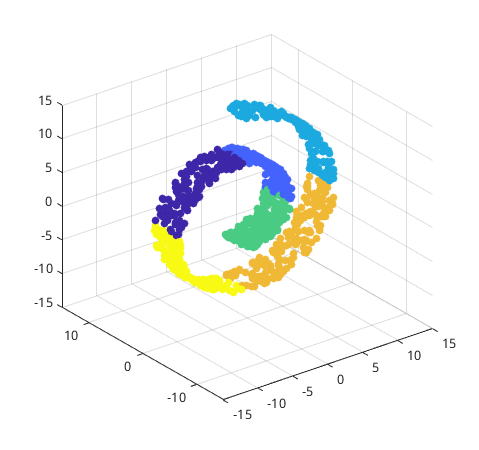
\includegraphics[width=0.7\linewidth]{images/swiss_roll.png}
    \caption{Swiss roll dataset}
    \label{swiss}
\end{figure}

\begin{figure}[H]
    \centering
    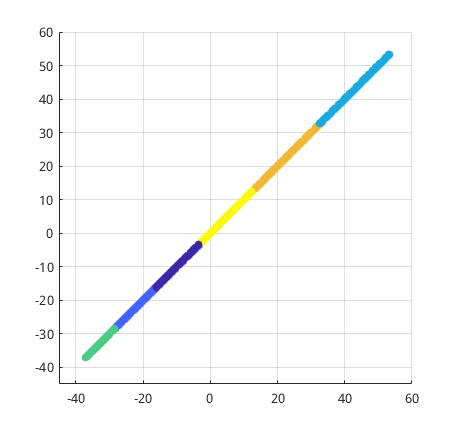
\includegraphics[width=0.6\linewidth]{images/swiss_roll_result.png}
    \caption{Swiss roll dataset reduced}
    \label{swiss_res}
\end{figure}

\begin{figure}[H]                                                                
    \centering                                                                   
    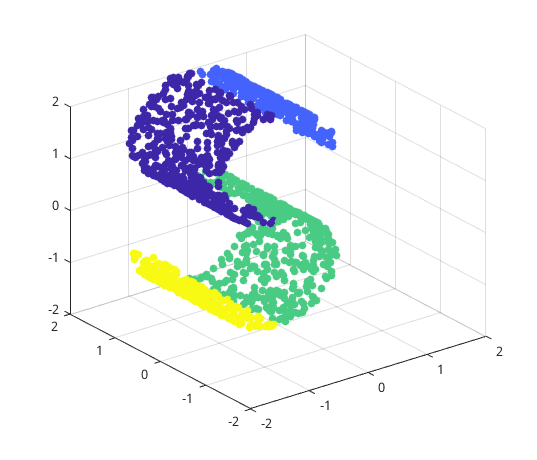
\includegraphics[width=0.9\linewidth]{images/s_curve.png}                    
    \caption{S curve dataset}                                                    
    \label{s_curve}                                                              
\end{figure}                                                                     
                                                                                 
\begin{figure}[H]                                                                
    \centering                                                                   
    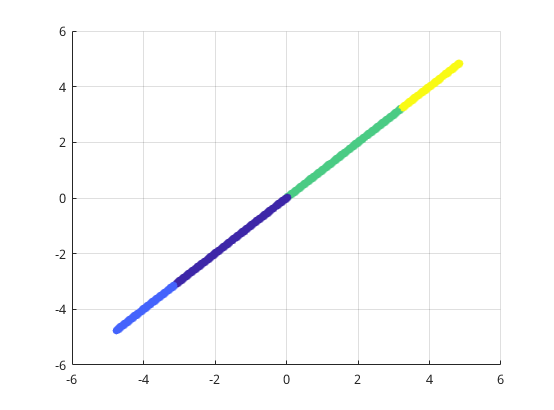
\includegraphics[width=0.9\linewidth]{images/s_curve_result.png}             
    \caption{S curve dataset reduced}                                            
    \label{s_curve_res}                                                          
\end{figure}

\section{Conclusions}

In this work a theorical and practical development of the multidimensional
scaling method was conducted. During the process it was found that what seemed like
a fairly complicated problem, can be simplified to simple matrix operations
with the help of some concepts from linear algebra. Thanks to that theorical
framework, the construction of a relatively simple algorithm that can detect
low dimensional manifolds embedded in multidimensional spaces became possible.
The results shown that this technique has the ability to make
contributions to the analysis proces of multidimensional datasets by
simplifying its features but preserving the intrinsic structure. Finally, as
future work, this method can be improved by creating new ways to compute the
matrix $D^x$. It would be interesting to implement this method using GPU
computations to improve its performance and use it as a mechanism of
data preprocessing in machine learning algorithms.

\section{Apendix}

    \subsection{Proof of the relationship between the norm and the trace} \label{norm_trace}

    \begin{equation*}
        \begin{aligned}
            \lVert A \rVert^2 = \sum_{i=1}^n \sum_{j=1}^n A_{ij}^2
            \hspace{1cm}
            Tr(A) = \sum_{i=1}^n A_{ii}
        \end{aligned}
    \end{equation*}\\

    Consider a matrix B that is computed as $A^tA$

    \begin{equation*}
        B = A^tA
    \end{equation*}

    Then, an element of B can be computed as

    \begin{equation*}
        B_{ij} = \sum_{k=1}^n A_{ik}^t A_{kj} = \sum_{k=1}^n A_{ki} A_{kj} = (A^tA)_{ij}
    \end{equation*}

    Now, the trace of B will be

    \begin{equation*}
        \begin{aligned}
            Tr(B) &= T(A^tA)\\
                  &= \sum_{i=1}^n (A^tA)_{ii}\\
                  &= \sum_{i=1}^n \sum_{j=1}^n A_{ij}^t A_{ji}\\
                  &= \sum_{i=1}^n \sum_{j=1}^n A_{ji} A_{ji}\\
                  &= \sum_{i=1}^n \sum_{j=1}^n A_{ji}^2 \\
                  &= \sum_{i=1}^n \sum_{j=1}^n A_{ij}^2 = \lVert A \rVert^2 \\
        \end{aligned}
    \end{equation*}

    Hence

    \begin{equation*}
        \lVert A \rVert^2 = Tr(A^tA)
    \end{equation*}

    \subsection{Proof of the circular transformation of the trace} \label{circular_trace}

    Consider a matrix M which is the multiplication of matrices B and C

    \begin{equation*}
        M = BC
    \end{equation*}

    Then an element of M is computed as

    \begin{equation*}
        M_{ij} = \sum_{k=1}^n B_{ik} C_{kj} = BC_{ij}
    \end{equation*}

    Now, the trace of M will be

    \begin{equation*}
        \begin{aligned}
            Tr(M) &= Tr(BC)\\
                  &= \sum_{i=1}^n BC_{ii}\\
                  &= \sum_{i=1}^n \sum_{j=1}^n B_{ij} C_{ji}\\
                  &= \sum_{i=1}^n \sum_{j=1}^n C_{ij} B_{ji}\\
                  &= \sum_{i=1}^n CB_{ii}\\
                  &= Tr(CB)
        \end{aligned}
    \end{equation*}

    Hence

    \begin{equation*}
        Tr(BC) = Tr(CB)
    \end{equation*}

    \subsection{Relationship between transpose and inverse of an othogonal matrix}
    \label{orthogonal}

    Consider an orthogonal matrix $Q$,

    \[
        Q =
        \begin{bmatrix}
             |  &        &  | \\
            q_1 & \cdots & q_n\\
             |  &        &  | \\
        \end{bmatrix}
    \]

    Since is orthogonal the following expression holds

    \[
        q_i q_j =
        \begin{cases}
           0 & i \neq j \\
           \lVert q_i \rVert & i = j
        \end{cases}
    \]

    And then

    \[
        Q^t Q =
        \begin{bmatrix}
             - q_1^t - \\
               \vdots  \\
             - q_n^t - \\
        \end{bmatrix}
        \begin{bmatrix}
             |  &        &  | \\
            q_1 & \cdots & q_n\\
             |  &        &  | \\
        \end{bmatrix}
    \]
    \[
        =
        \begin{bmatrix}
            q_1^t q_1 & \cdots & q_1^t q_n \\
              \vdots  & \ddots &  \vdots   \\
            q_n^t q_1 & \cdots & q_n^t q_n \\
        \end{bmatrix}
        =
        \begin{bmatrix}
          \lVert q_1 \rVert &         0         & \cdots &         0    \\
                  0         & \lVert q_2 \rVert & \cdots &         0    \\
               \vdots       &       \vdots      & \ddots &       \vdots \\
                  0         &         0         & \cdots & \lVert q_n \rVert \\
        \end{bmatrix}
    \]

    Which implies that if all the vectors of $Q$ have a length of one ($Q$ is
    orthonormal), then

    \begin{equation*}
        Q^t Q = I
    \end{equation*}

    And if $Q$ is also square, then

    \begin{equation*}
        Q^t = Q^{-1}
    \end{equation*}

    \subsection{Spectral decomposition for symmetric matrices} \label{spectral_decomp}

    Consider a symmetric matrix $A$, then this matrix will have $n$ orthogonal
    eigenvalues. Then build a new matrix $S$ that will contain the eigenvalues of
    $A$ as columns.\\

    Now from the definition of eigenvalues and eigenvectors

    \begin{equation*}
        A \mu = \lambda \mu
    \end{equation*}

    If $\mu$ is replaced with $S$ the result would be

    \[
        A S = A
        \begin{bmatrix}
              |   &        &   |  \\
            \mu_1 & \cdots & \mu_n\\
              |   &        &   |  \\
        \end{bmatrix}
        =
        \begin{bmatrix}
             & - x_1^t - &\\
             &  \vdots   &\\
             & - x_n^t - &\\
        \end{bmatrix}
        \begin{bmatrix}
              |   &        &   |  \\
            \mu_1 & \cdots & \mu_n\\
              |   &        &   |  \\
        \end{bmatrix}\\
    \]
    \[
        =
        \begin{bmatrix}
            x_1^t \mu_1 & \cdots & x_1^t \mu_n\\
               \vdots   & \ddots &   \vdots   \\
            x_n^t \mu_1 & \cdots & x_n^t \mu_n\\
        \end{bmatrix}
        =
        \begin{bmatrix}
                    |       &        &         |      \\
            \lambda_1 \mu_1 & \cdots & \lambda_n \mu_n\\
                    |       &        &         |      \\
        \end{bmatrix}\\
    \]
    \[
        =
        \begin{bmatrix}
               |  &        &   |  \\
            \mu_1 & \cdots & \mu_n\\
               |  &        &   |  \\
        \end{bmatrix}\\
        \begin{bmatrix}
            \lambda_1 &      0    & \cdots &   0 \\
                0     & \lambda_2 & \cdots &   0 \\
              \vdots  &   \vdots  & \ddots & \vdots \\
                0     &      0    & \cdots & \lambda_n \\
        \end{bmatrix}\\
    \]

    So, if a new matrix $\Lambda$ is defined as a diagonal matrix that contains
    the eigenvalues of $A$, then the computation can be expressed as

    \begin{equation*}
        A S = S \Lambda
    \end{equation*}

    And, since $S$ is invertible

    \begin{equation*}
        A = S \Lambda S^{-1}
    \end{equation*}

    Finally, as shown in section \ref{orthogonal}, the inverse of an orthonormal
    matrix is its traspose, then A can be expressed as

    \begin{equation*}
        A = S \Lambda S^t
    \end{equation*}

\bibliographystyle{unsrt}
\bibliography{Article_mds}

\end{document}
